\documentclass{StdTemplate} % use larger type; default would be 10pt
\DeclareSIUnit\dB{\text{dB}}
\DeclareSIUnit\oct{\text{oct}}
\DeclareSIUnit\in{\text{in}}
\DeclareSIUnit\ft{\text{ft}}

\title{Review of the Findings and Accomplishments Resulting from Constuction of a Set of Full Range Speakers and Their Supporting Hardware}
\author{c3h99}
\date{\today}
\HeaderLeft{\thetitle}
\HeaderRight{\thesection}

\begin{document}
\TitlePage
%
\begin{abstract}
A three-way, floor standing loudspeaker featuring an active crossover was designed to have a flat frequency response over the majority of the acoustic range. A measured system response from \SIrange{20}{20000}{\hertz} was achieved to a flatness of \SI{\pm 5}{\dB} using minDSP’s UMIK-1 USB microphone.
\end{abstract}
%
%\section*{Frontmatter}
%
\subsection{Disclaimer}
I am not an expert, and this content should not be construed as professional advice. All measurements are made in adverse, non-ideal conditions with uncalibrated equipment, often of consumer grade. All content, regardless of technical appearance, should be treated as the opinion of an unskilled monkey who has broken free of his cage and is intent on escaping (humorously referred to as the author). No guarantees of quality, reproducibility, or success are made. No warranty of any kind is provided and the author(s) are not liable for any claim(s) or consequence(s) which may arise.\par
%
\subsection{Forward}
Like many projects undertaking stems from a personal curiosity about the subjects herein presented and a fundamental desire to design and build. Only after trying to do something, we learn how woefully incomplete and inaccurate are the writings and descriptions of experts. Despite these limitations, we must aspire to learn from others and, then, from ourselves.\par

\section{Introduction}
A simple goal of building a simple pair of speakers has grown into a significant undertaking. The (intermediate) results continue to be satisfactory. Discussion of the design process, findings, and results are contained in the sections to follow.\par
\section{Loudspeaker Design}
%
\subsection{Driver Selection}
A three-way design was chosen for its added technical complexity and bass extension potential. A semi-scientific selection process was used to determine the individual speaker elements (drivers) for use in the loudspeaker design. Drivers were chosen to maximize agreement between rated sound pressure levels (SPL). Crossover points were loosely defined for the tweeter to operate at frequencies in the \si{\kilo\hertz} range and above, the subwoofer to operate at frequencies below hundreds of \si{Hz} and the mid to operate in the range between. Agreement in output phase was not considered but is encouraged in future efforts. Interference effects between the drivers resulting from phase differences are attributed to undesired difficulty in crossover design and implementation. \par
%
Prior experience with ribbon tweeters motivated limited selection to within the topology. SPL response graphs show them comparing highly favorably to conventional tweeters. The majority of the driver budget was allocated to the tweeters, with the minority being afforded to subwoofers. Larger subwoofer drivers were chosen for their const and frequency response. An analytical optimum of these factors appears to exist in the range of 10 to 12 inch drivers. The mid was chosen less scientifically but has proven to be an exceptional driver. Based on prior experience stemming from their popularity in hobbyist communities, drivers were purchased from PartsExpress whom caters to car audio and DIY speaker enthusiasts. Selected parts are noted in \Figure{sp_drivers}.\par
%
\begin{figure}[h!]
\centering
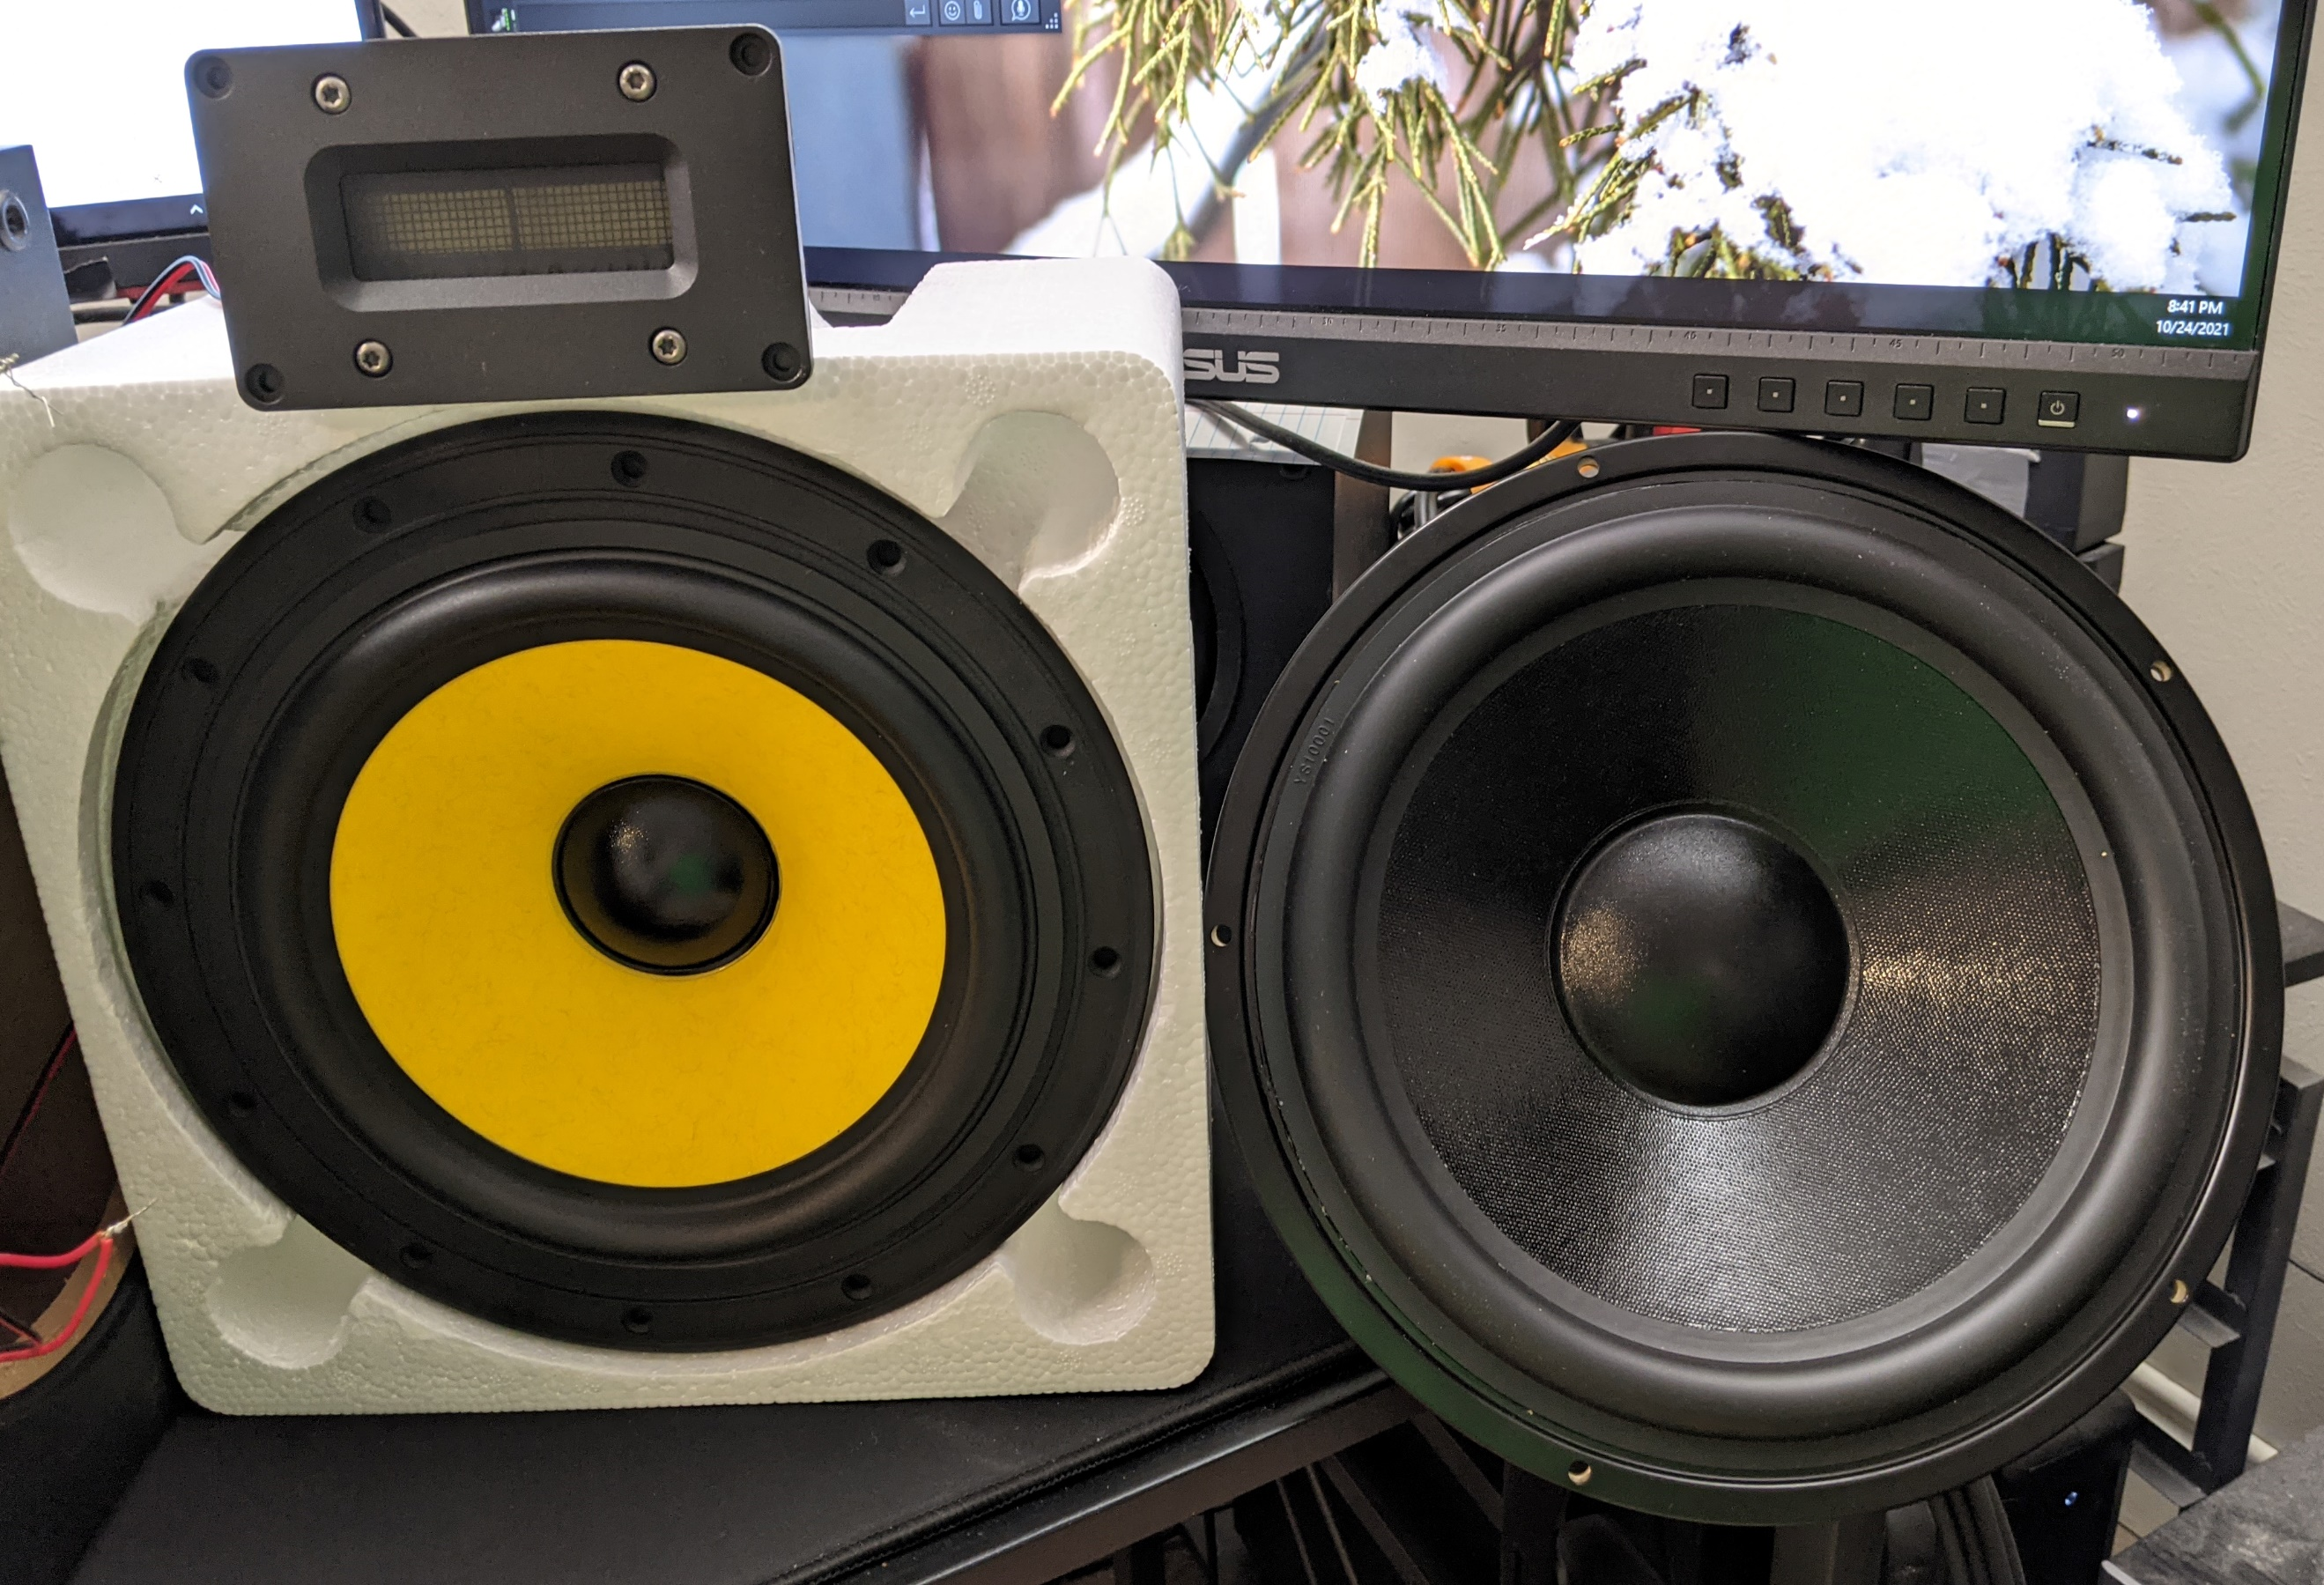
\includegraphics[width = 5.3 in]{Images/sp_drivers.jpeg}
\caption{Selected drivers. Top left: (Ribbon tweeter) Fountek Neo X 2.0, Bottom left: (Mid-Bass) HiVi F8, Right: (Sub-Woofer) Dayton Audio SD270-A, Not shown: (Passive Radiator) Dayton Audio DS270-PR 10- Visually similar to subwoofer. For size reference, the outer diameter of the sub-woofer is approximately 12 in. It should be noted that approximately \SI{17}{\gram} of mass is added to the subwoofer in the final implementation.}
\label{fig:sp_drivers}
\end{figure}
%
\subsection{Cabinet Design}
A preliminary series of designs were considered and modelled using the templates available within the freely publish WinISD modelling software. Curiosity regarding the efficacy and accuracy of these designs motived developing prototype cabinets from cheaply available materials. The author failed to understand that operation of the enclosure depends on the structure being a rigid enclosure which isolates the sound generated by the back of the driver from the sound generated by the front of the driver. In keeping with this mistake, a series of prototypes were made using extruded polystyrene (XPS) and PVC tubing cut to length as experimental port material. The limited stiffness of the material allowed limited gains from enclosing the back of the driver, but the impact of porting was not audibly noticeable. Images of this failed approach are included as \Figure{sp_xps_proto}.\par 
%
\begin{figure}[h!]
\centering
\subfloat[\centering Raw materials.]{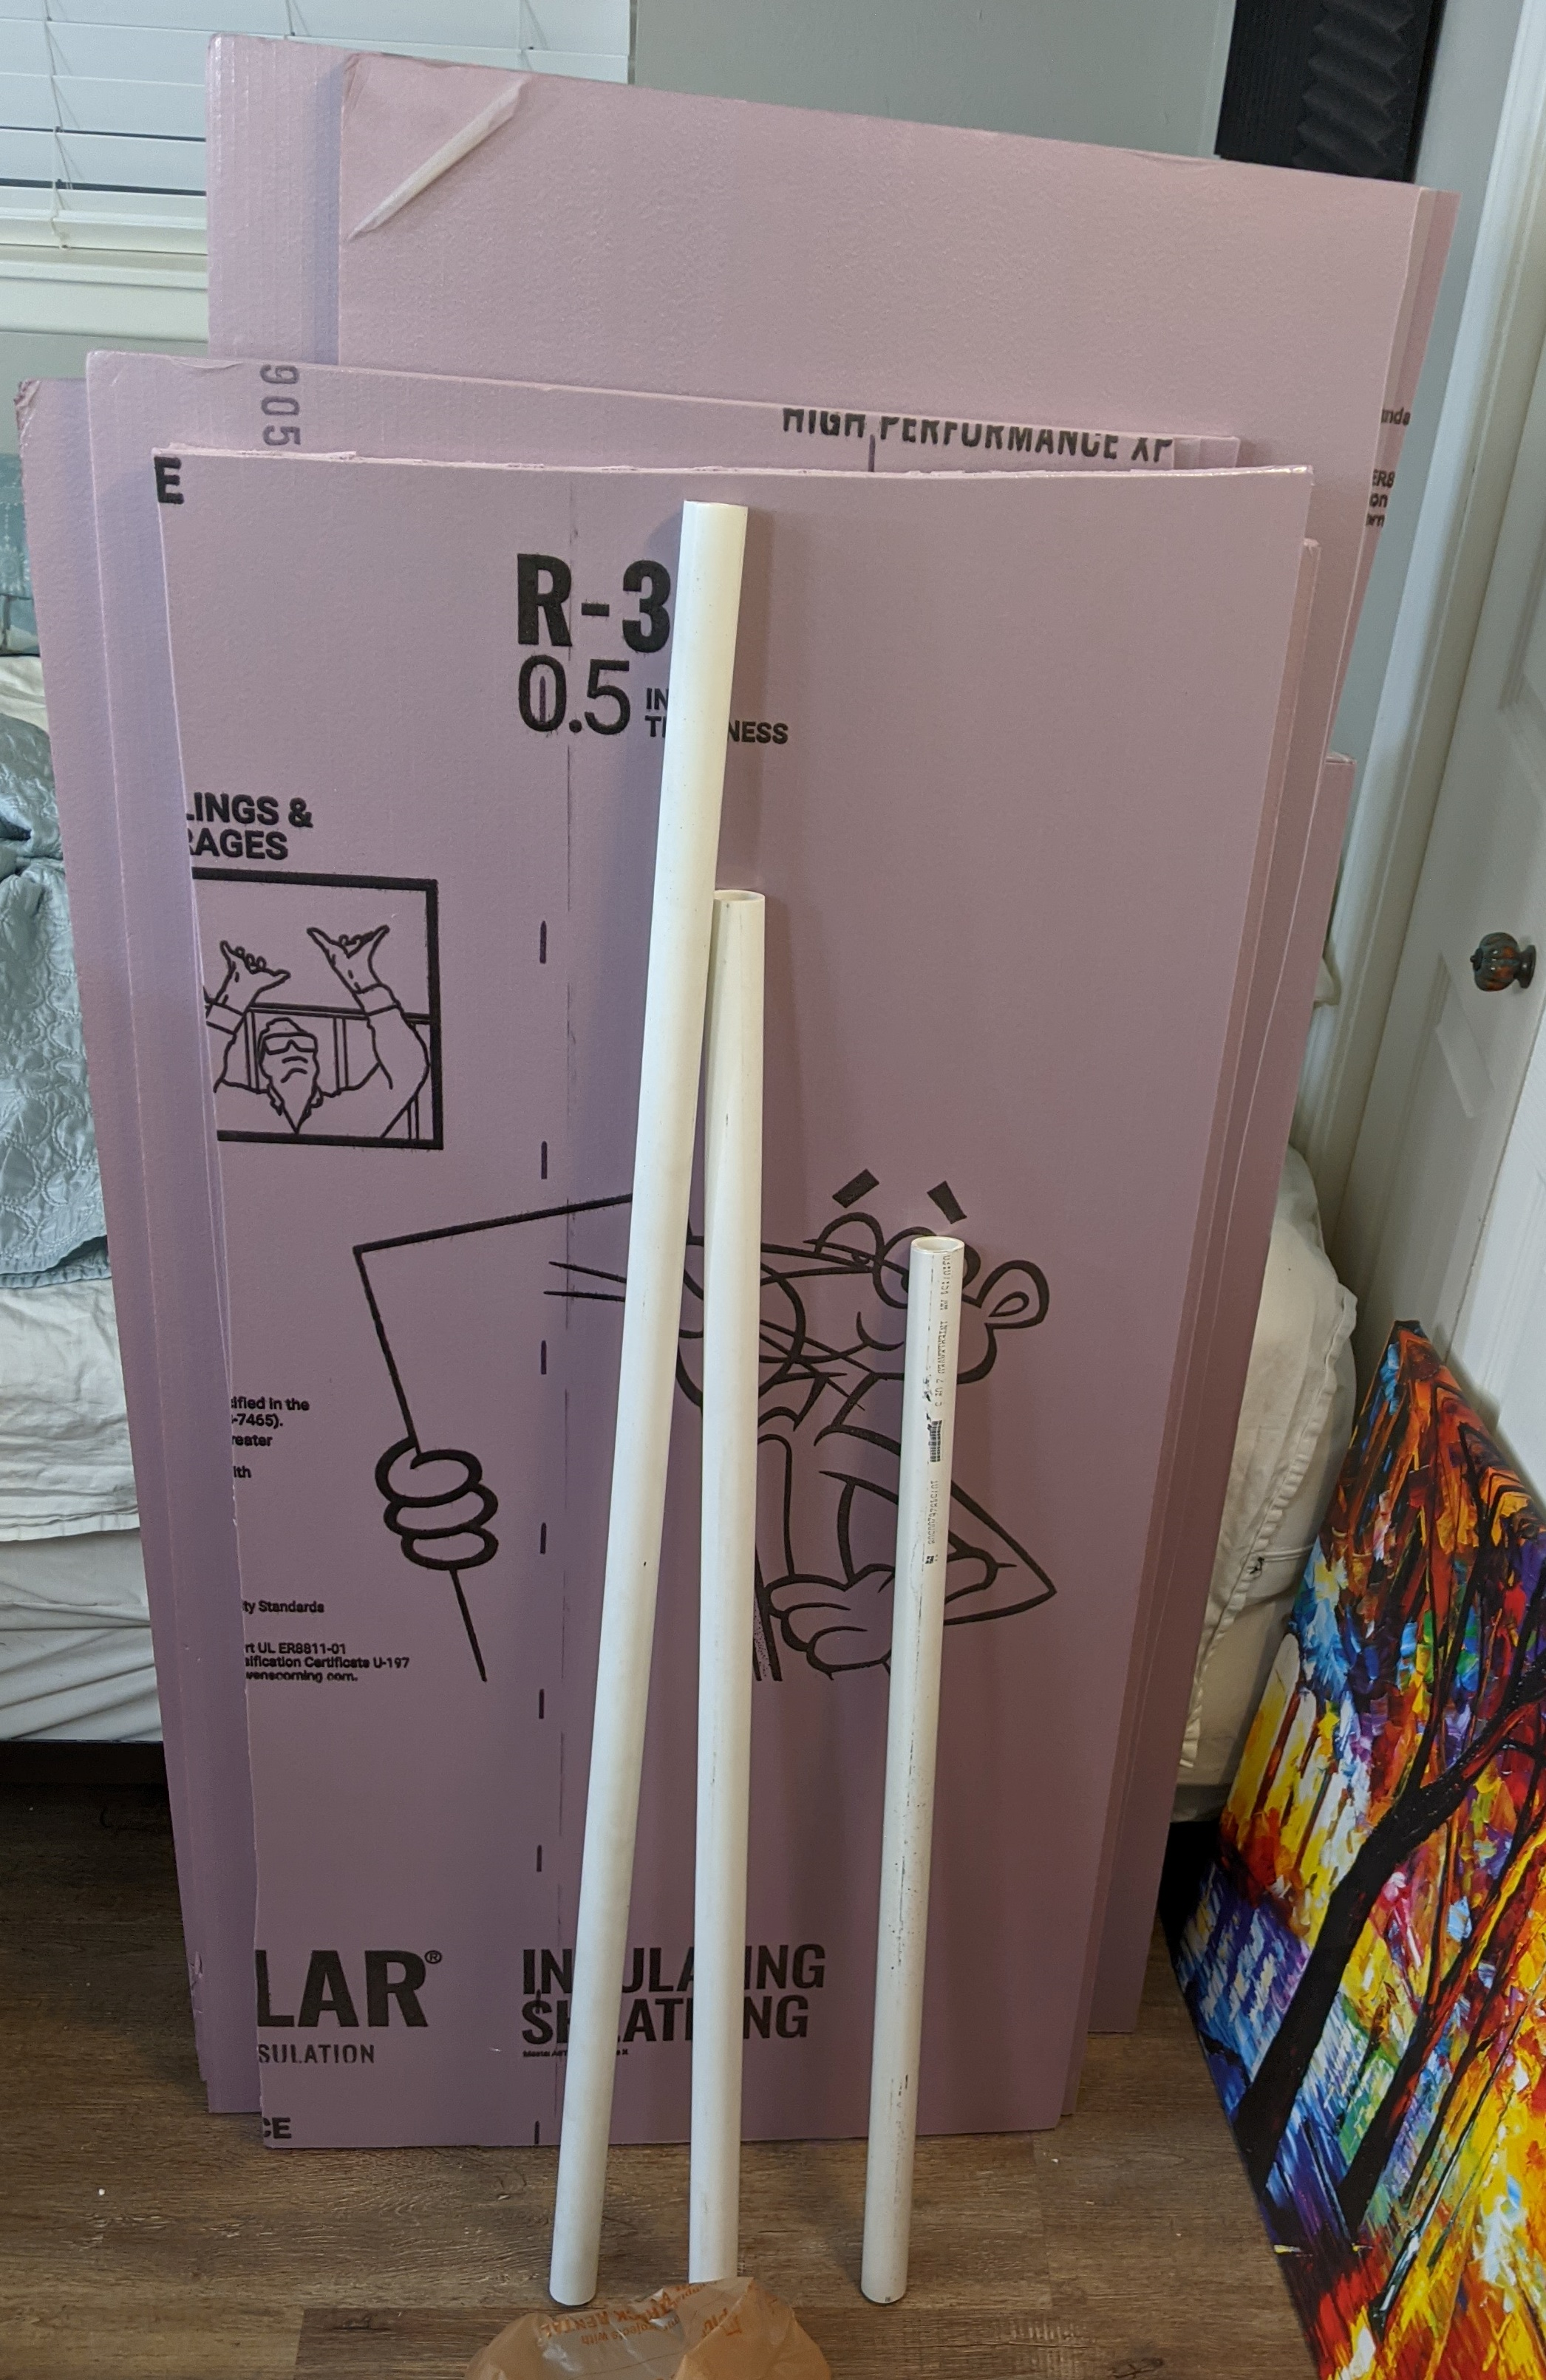
\includegraphics[height = 3.5 in]{Images/sp_xps_proto1.jpeg}}
\qquad
\subfloat[\centering Constructed cabinet.]{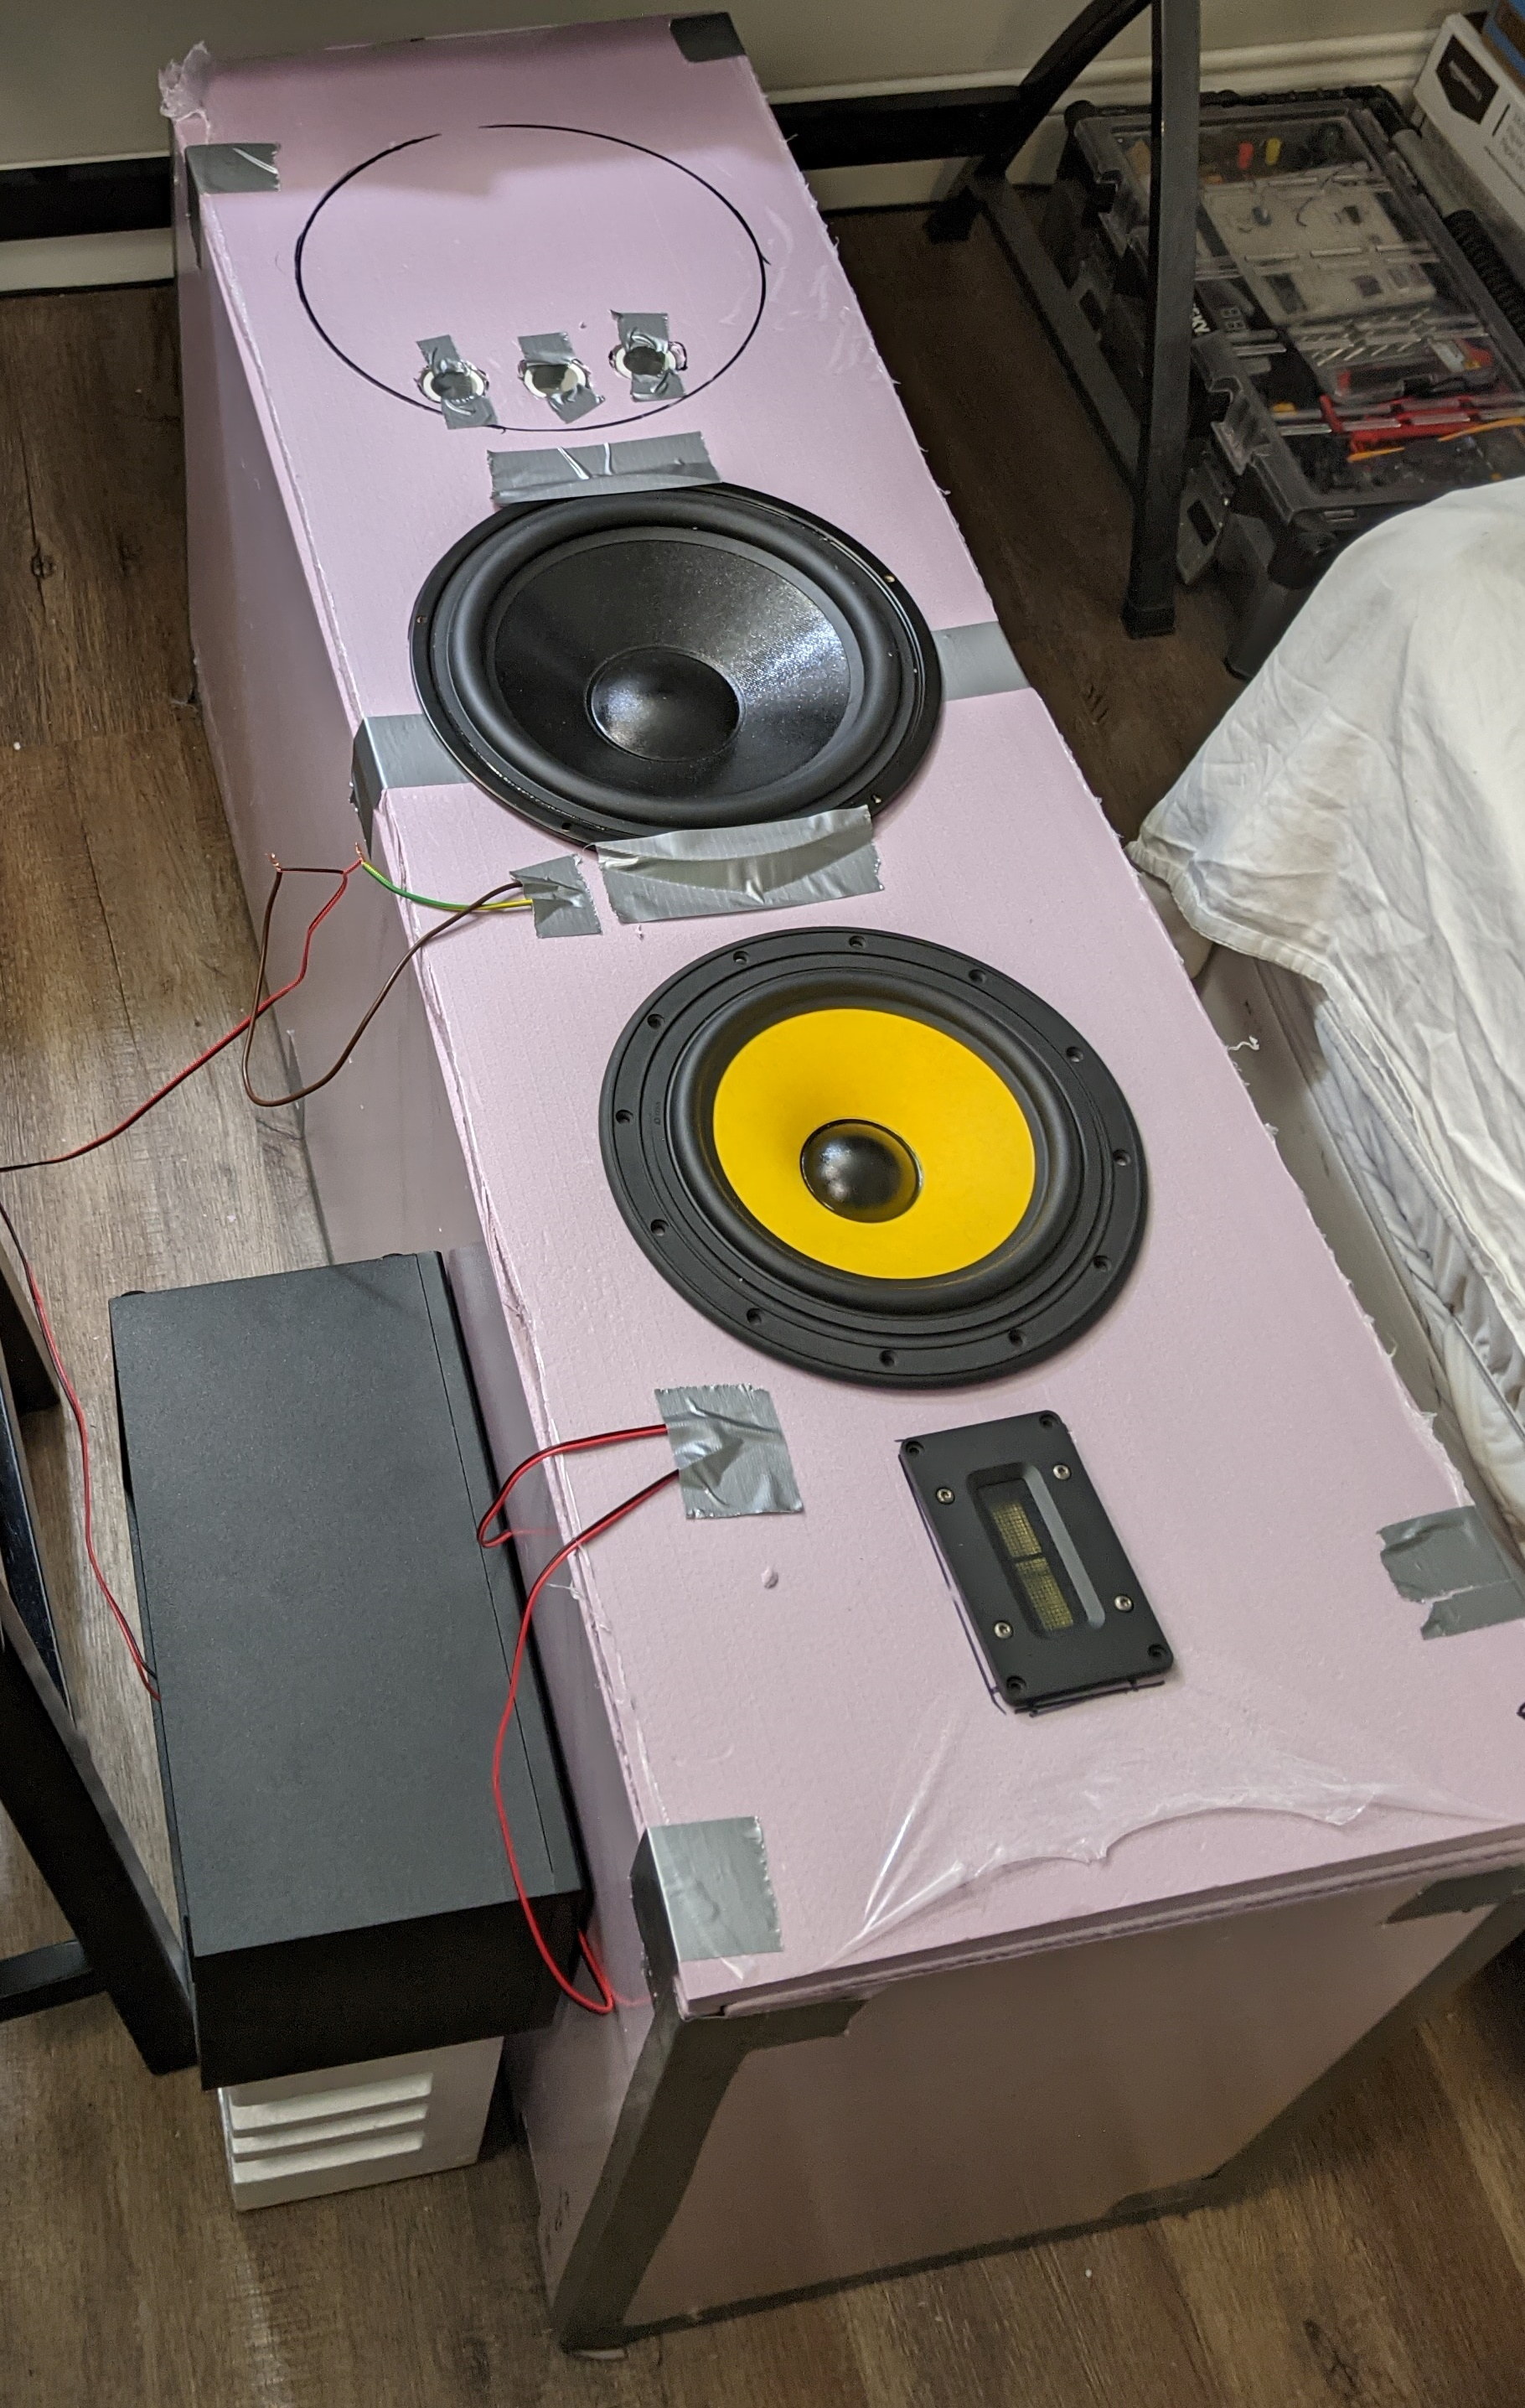
\includegraphics[height = 3.5 in]{Images/sp_xps_proto2.jpeg}}
\caption{Initial cabinet prototype constructed from $\frac{1}{2}$~in thick Owens-Corning Foamular\textsuperscript{\textregistered} extruded polystyrene (XPS) insulation. The resulting construction was of very limited stiffness (additional effort would be required to reach a reasonable level of stiffness). PVC pipe was trimmed to desired length to be used as inexpensive venting/ports. Some improvement in bass response was observed with XPS. However, the improvement over enclosureless/baffleless operation was marginal and insubstantial compared to the final wooden construction.}
\label{fig:sp_xps_proto}
\end{figure}
%
Cabinet porting in the form of a passive radiator was chosen out of curiosity. Preliminary simulations in WinISD suggested comparable performance was possible, though it readily showed that the cutoff of the passive radiator was far more aggressive than a ported design. However, it was not subjected to port noise in the form of resonances and chuffing which must be accounted for in a ported design. Less is readily available about passive radiator designs, but templates for simple chambers exist.\par
%
The final design was tuned for ease of manufacturing. The full height of the speaker was \SI{4}{ft} to allow the width of a full sheet of Birch plywood to define a major length and provide a reference edge for most of the subsequent cuts. Some 2X4’s were ripped to produce \SI{1.5}{\in} square stock to reinforce the vertical seams of the cabinet interior and to provide mounting aids for the top and bottom faces (feature not included in the provided drawing). Annotated drawings are included as \Figure{sp_cad}. Constructing a pair of cabinets required approximately 1.5 full sheets of plywood.\par
%
\begin{figure}[h!]
\centering
\subfloat[\centering CAD Rendering.]{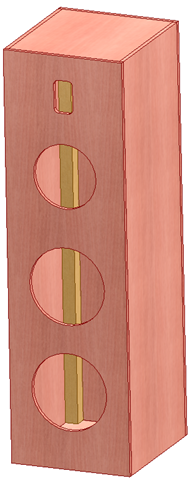
\includegraphics[height = 3.5 in]{Images/sp_cad_view.png}}
\qquad
\subfloat[\centering CAD Drawing. All units in inches.]{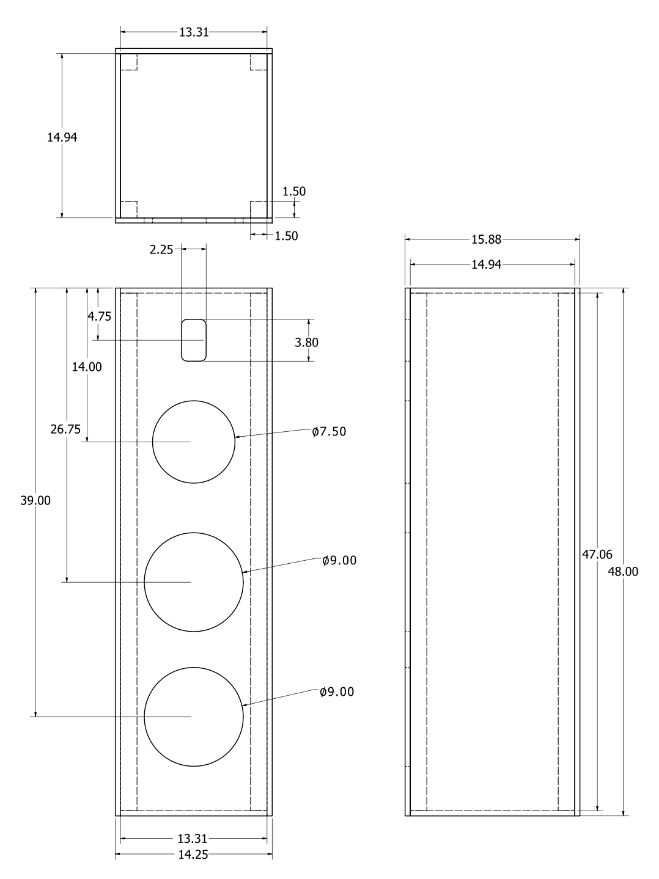
\includegraphics[height = 3.5 in]{Images/sp_cad_drawing.png}}
\caption{Cabinet design. Details are based on final measured results, rather than being the construction reference. Neglecting driver displacement, interior volume is approximately \SI{5.17}{\ft^3}}
\label{fig:sp_cad}
\end{figure}
%
\subsection{Cabinet Construction}
Intermediate construction steps are depicted in \Figure{sp_faces} where the front and back panels are being assmbled. Panels were made of $\frac{1}{2}$~\si{\in} nominal Birch plywood with pine vertical supports interior to the volume. The vertical supports were clamped and glued to the front/rear face panels during the curing process. Afterwards, holes for the drivers and passive radiator were free-hand cut with a jig saw.\par
%
\begin{figure}[h!]
\centering
\subfloat[\centering Front/Back panels wailting for glue to dry.]{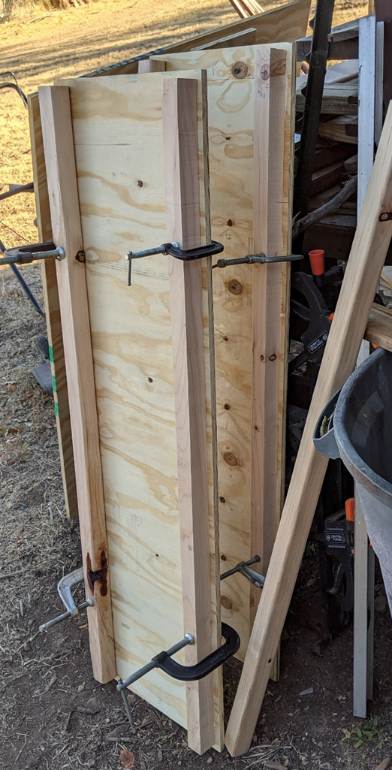
\includegraphics[height = 3.5 in]{Images/sp_face_construction1.png}}
\qquad
\subfloat[\centering Surface repair following cuts made to recieve speaker drivers.]{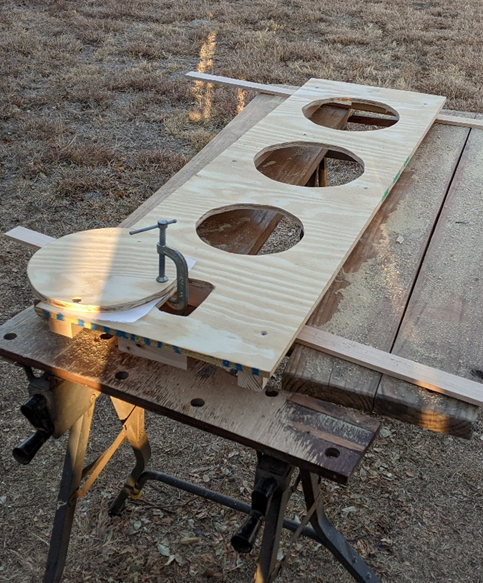
\includegraphics[height = 3.5 in]{Images/sp_face_construction2.png}}
\caption{Intermediate construction of cabinets.}
\label{fig:sp_faces}
\end{figure}
%
Cabinets were stained with two coats of Minwax\textsuperscript{\textregistered} PolyShades\textsuperscript{TM} Natural Cherry stain (and polyurethane) with a satin finish. The included polyurethane makes the stain incompatible with other stains and generally impeded the intended construction, where the cherry was intended to warm the light tones of Minwax\textsuperscript{\textregistered} Get Stain in a Mahogany finish. In total, the two coats consumed the better part of a quart of stain to finish both cabinet exteriors. Stain results are depicted in \Figure{sp_stain}.\par
%
\begin{figure}[h!]
\centering
\subfloat[\centering Cabinets stained and curing. ]{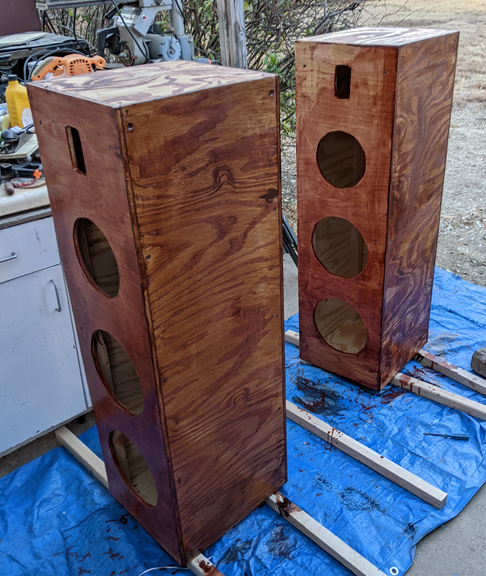
\includegraphics[height = 3.5 in]{Images/sp_cabinate_stain.png}}
\qquad
\subfloat[\centering Cabinets with drivers added (bottom element is passive radiator)]{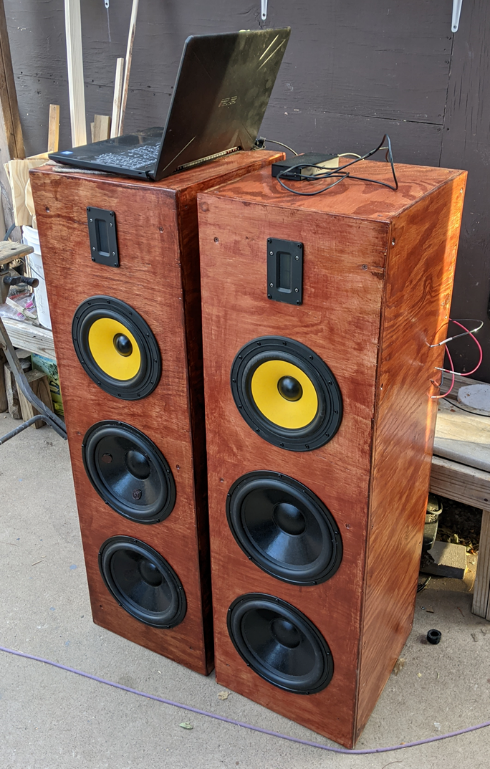
\includegraphics[height = 3.5 in]{Images/sp_assembled.png}}
\caption{Intermediate construction of cabinets.}
\label{fig:sp_stain}
\end{figure}
%
Initially the cabling was left as a un-terminated “pig tail”, but later a “Cable Matters” brand “double gang speaker wall plate for 6 speakers” was purchased and re-purposed as a feedthrough. The internal wires were directly connected, which required the plate to be mounted internally leaving access only to the banana plugs from the rear. The process did not cut cleanly, and results are shown in \Figure{sp_binding_posts}.\par
%
\begin{figure}[h!]
\centering
\subfloat[\centering Binding posts installed and sealed with epoxy. View from speaker interrior.]{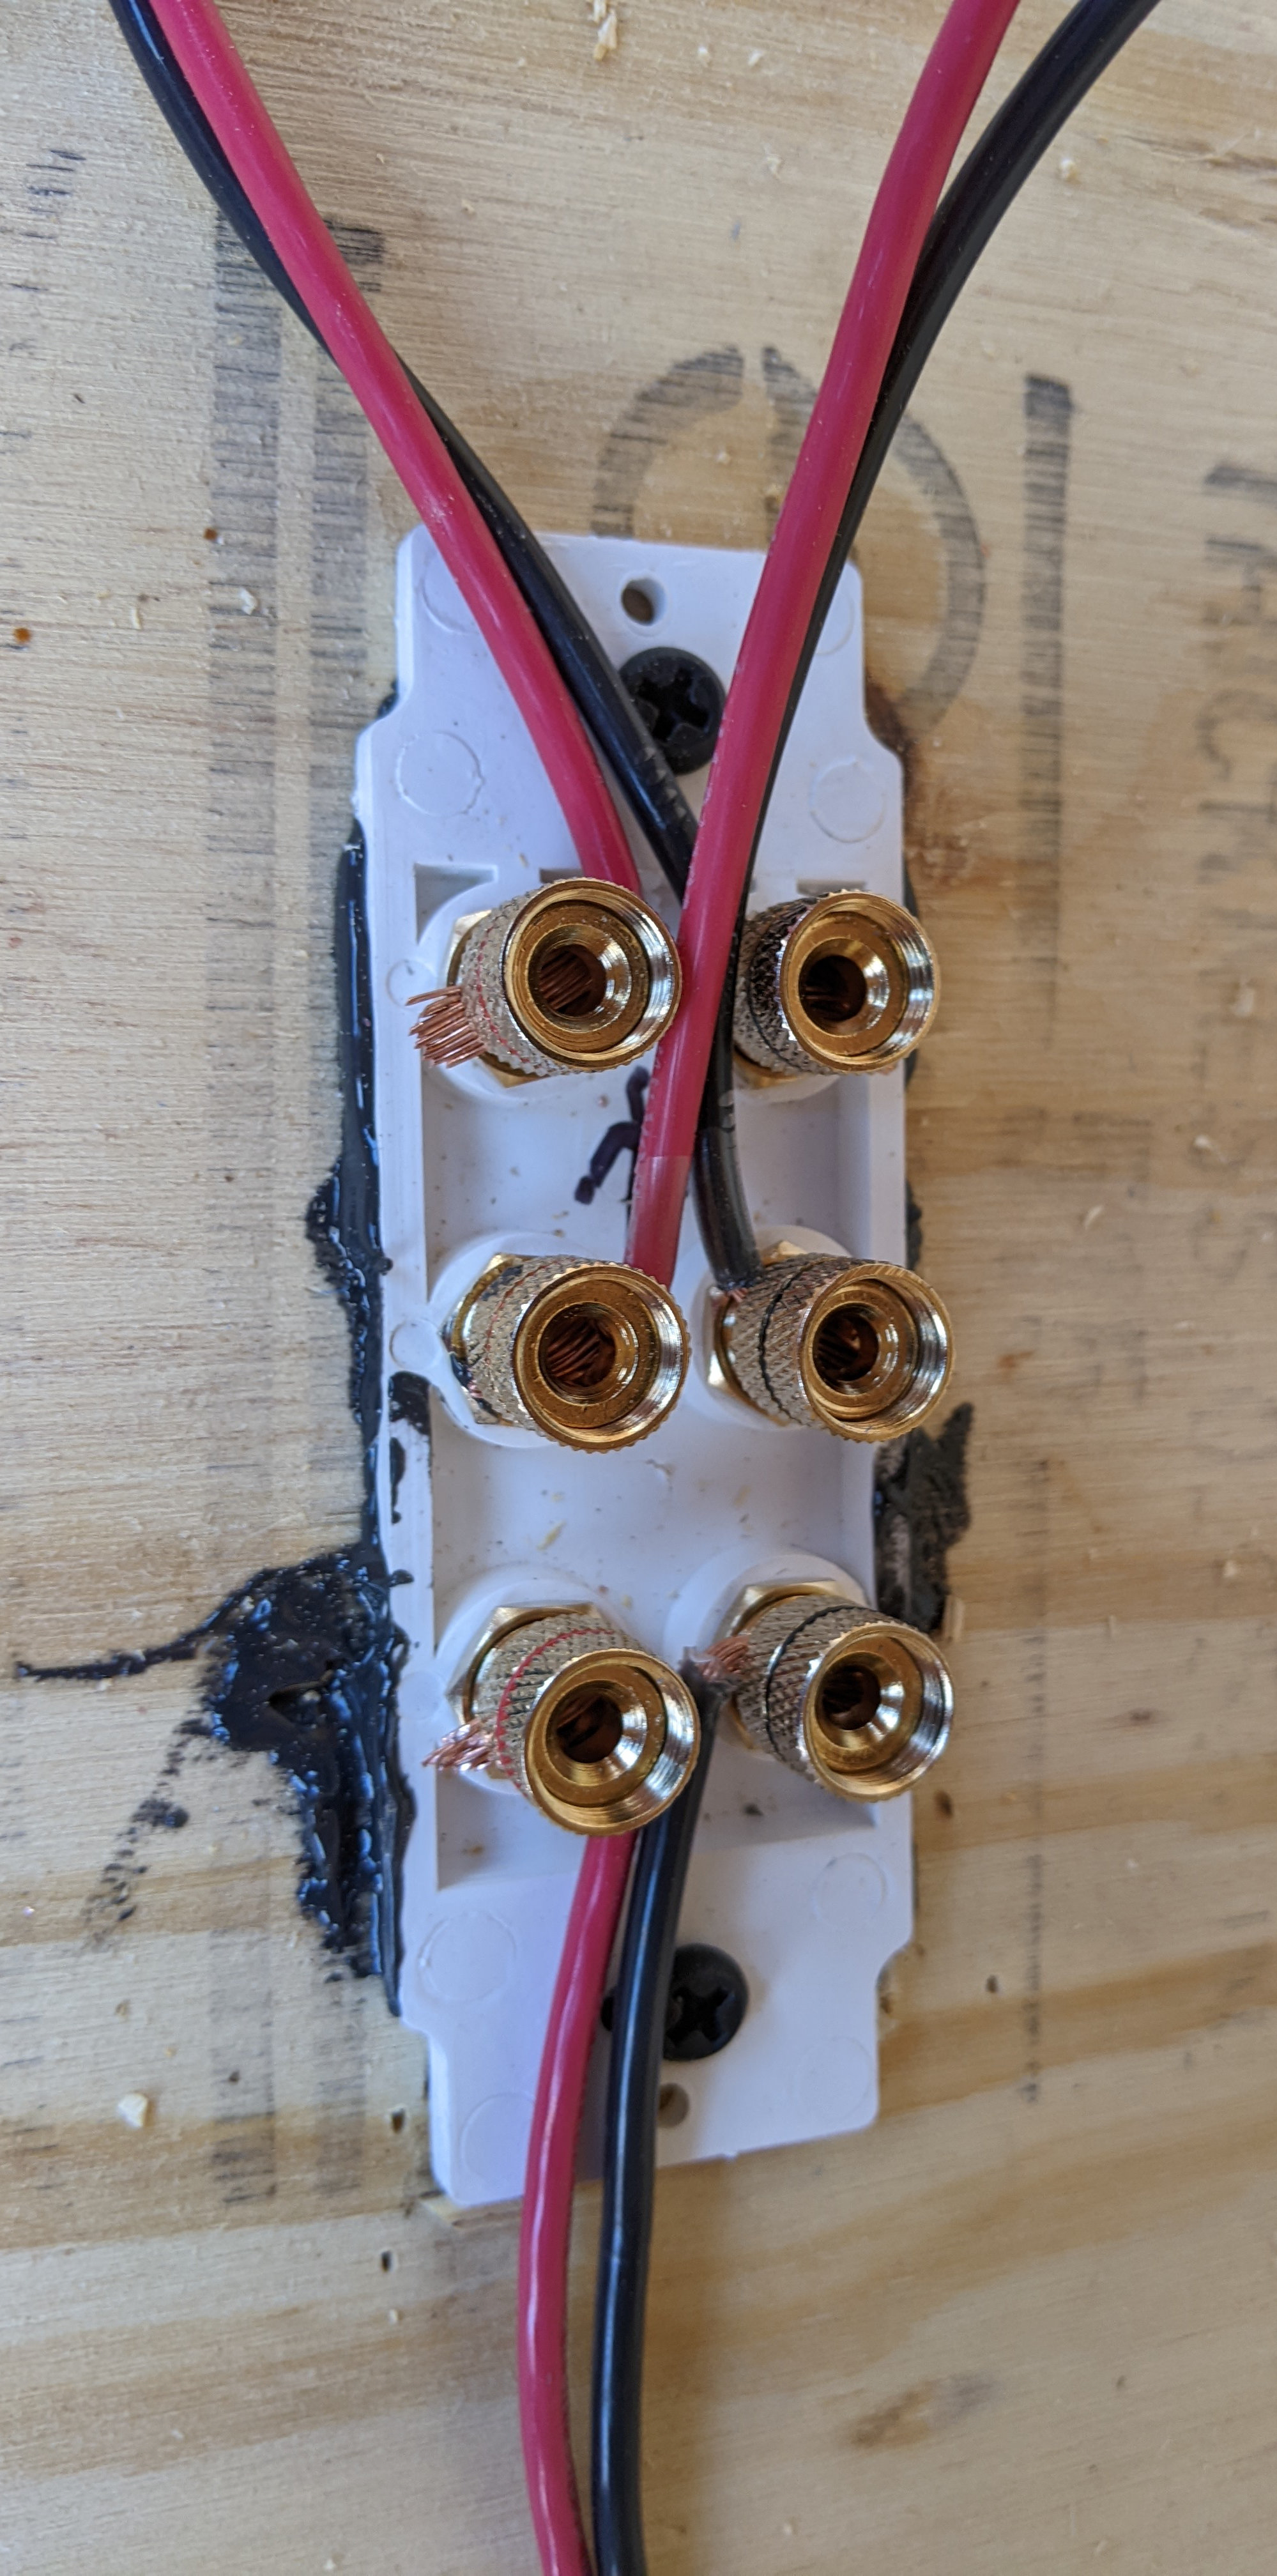
\includegraphics[height = 3.5 in]{Images/sw_wall_plate1.jpg}}
\qquad
\subfloat[\centering Binding posts as viewed from speaker rear. Tearout was undesirable, but out of sight during regular use.]{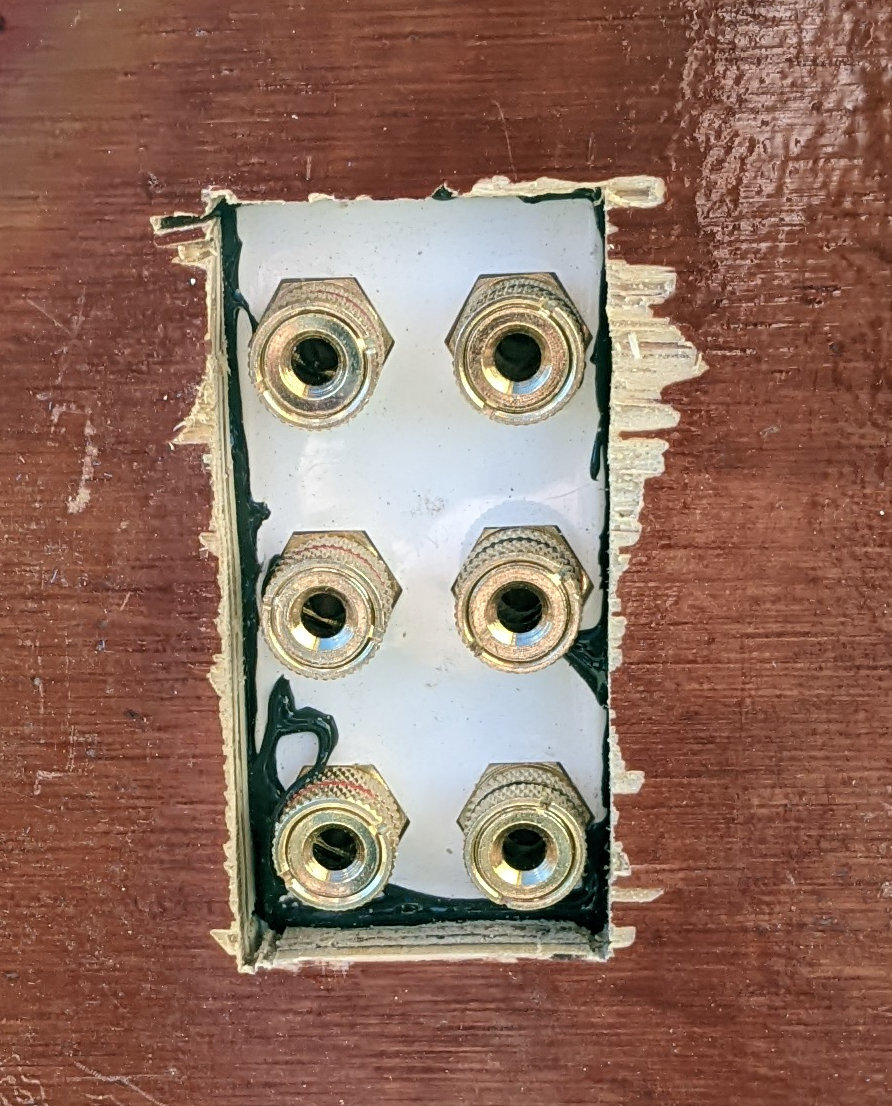
\includegraphics[height = 3.5 in]{Images/sw_wall_plate2.jpg}}
\caption{Added binding posts.}
\label{fig:sp_binding_posts}
\end{figure}
%
A low dispersion, \SI{47}{\uF}, polymer capacitor was located internally, in-series with the tweeter to protect from shorting under DC conditions. This is purportedly an issue of such devices, however, the author was unwilling to test either tweeter to destruction to verify the claim. The internal cabling configured and fastened as is shown in \Figure{sp_cabling}.\par
%
\begin{figure}[h!]
\centering
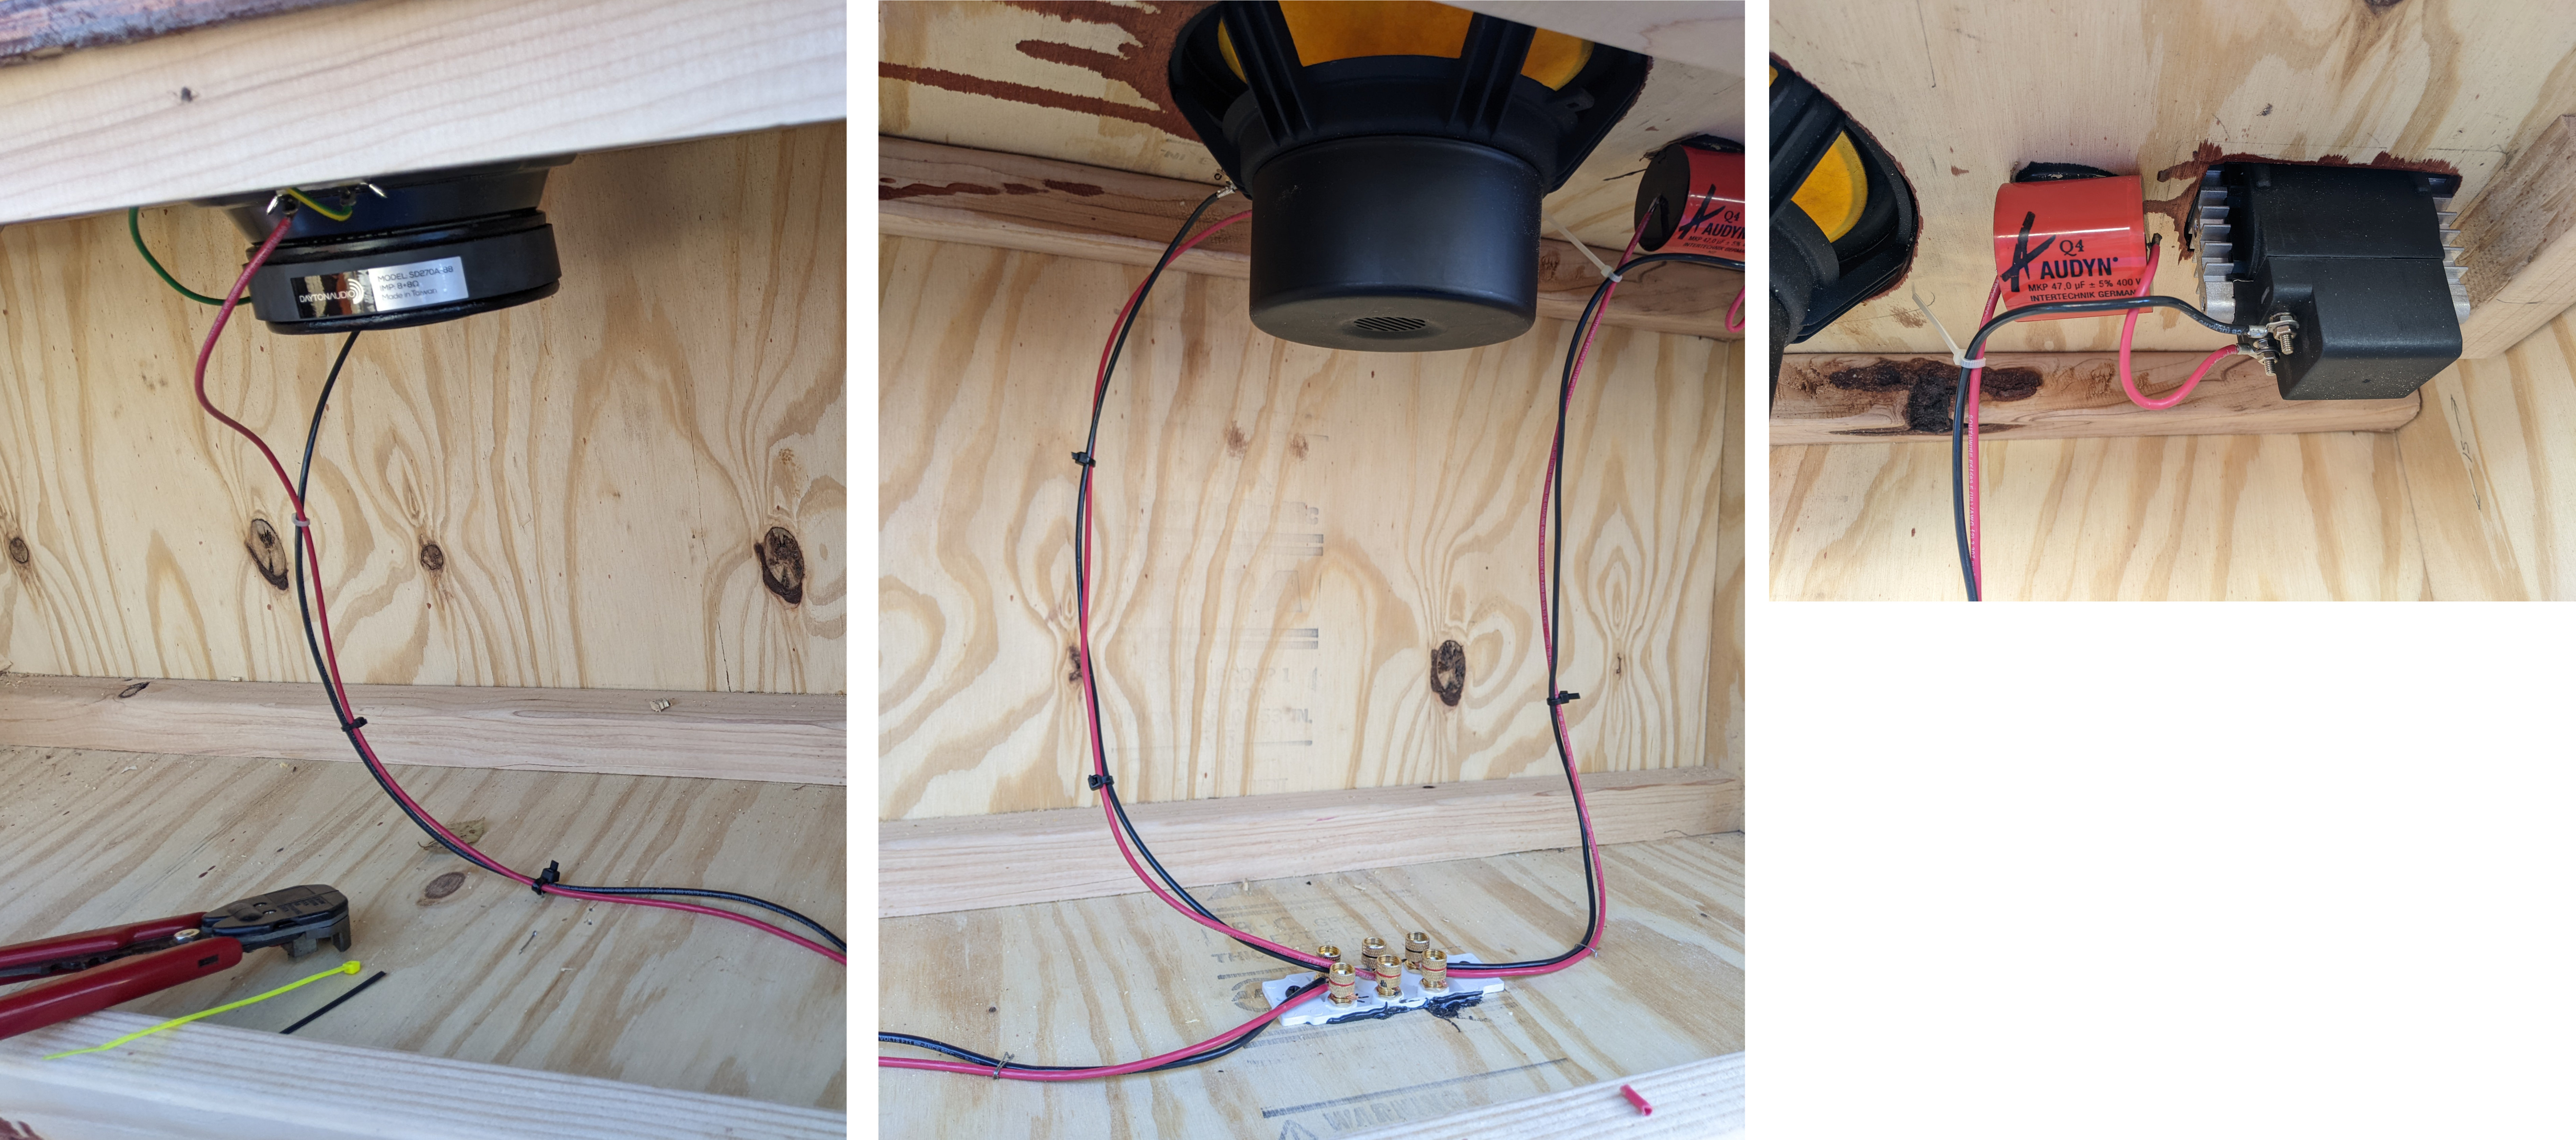
\includegraphics[width = 7 in]{Images/sp_int_collage.jpg}
\caption{Internal cabling of loudspeakers. Pairs of conductors where kept close to minimized inductance, and trimmed to length where possible.}
\label{fig:sp_cabling}
\end{figure}
%
\subsection{Initial Measurements and Tuning}
The loudspeakers were tested in an outdoor, semi-open region with a hard concrete floor and significant ambient noise. The system was powered using an old Denon home theater receiver in a fully active configuration. A total of 6 channels are needed to drive both loudspeakers. A pair of MiniDSP 2X4 HD digital signal processors were configured to provide software cross-over functionality for ease- and rapidity- of prototyping. One module was dedicated to each loudspeaker. The configuration for one speaker was mirrored to the other module. This methodology proved to be effective, and measurements showed similar performance across the two loudspeakers. Initial test tones were generated using the integrated soundcard of a laptop computer. Given the quoted response of the tweeters, it is strongly believed that the laptop exhibited a low-order low-pass filter with cutoff near \SI{17}{\kilo\hertz}.\par
%
The SPL response of the individual drivers (in new condition) was measured following their installation into the cabinet. Again, the MiniDSP UMIK-I was used to measure the response (in a high noise floor environment) with the Dayton Audio DATS v3 powering the individual drivers. Drivers not powered were shorted to approximate a low-impedance source of their own. The tweeter measured a SPL well below the \SI{95}{\dB} on-axis response that is quoted in the datasheet but exhibit the same general trends beyond \SI{1}{\kilo\hertz}. This likely is due to difference in the absolute accuracy of the microphone and the measurement setup. The subwoofer generally agrees with datasheet, with exception of the difference in absolute level. The mid disagreed the most with the datasheet. A predicted roll-off starting near \SI{100}{\hertz} was replaced with an extension well into \SI{30}{\hertz}. The cabinet may work well as a two-way system of tweeter and mid, possibly requiring the subwoofer and passive radiator as a pair of passive radiators. The bass extension is not predicted by WinISD when modeling the mid and a single passive radiator. These discrepancies may be attributable to the use of a single chamber for all cavities, and or the measurement conditions themselves. Responses are presented in \Figure{sp_measured_SPL_resp}.\par
%
The SPL response of the individual drivers (in new condition) was measured following their installation into the cabinet. Again, the MiniDSP UMIK-I was used to measure the response (in a high noise floor environment) with the Dayton Audio DATS v3 powering the individual drivers. Drivers not powered were shorted to approximate a low-impedance source of their own. The tweeter measured a SPL well below the \SI{95}{\dB} on-axis response that is quoted in the datasheet but exhibit the same general trends beyond \SI{1}{\kilo\hertz}. This likely is due to difference in the absolute accuracy of the microphone and the measurement setup. The subwoofer generally agrees with datasheet, with exception of the difference in absolute level. The mid disagreed the most with the datasheet. A predicted roll-off starting near \SI{100}{\hertz} was replaced with an extension well into \SI{30}{\hertz}. The cabinet may work well as a two-way system of tweeter and mid, possibly requiring the subwoofer and passive radiator as a pair of passive radiators. The bass extension is not predicted by WinISD when modeling the mid and a single passive radiator. These discrepancies may be attributable to the use of a single chamber for all cavities, and or the measurement conditions themselves. Responses are presented in \Figure{sp_measured_SPL_resp}.\par
%
\begin{figure}[h!]
\centering
\subfloat[\centering Overlayed Responses]{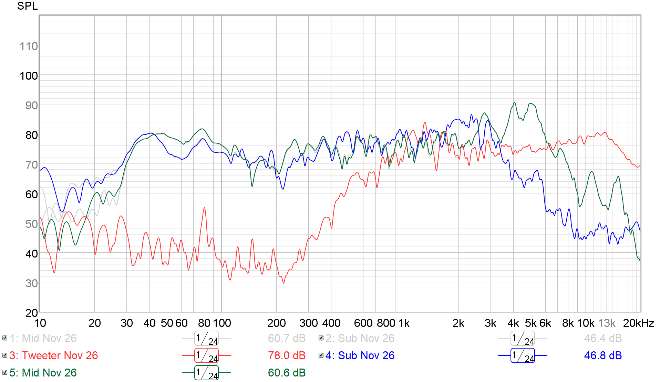
\includegraphics[width = 3 in]{Images/sp_spl_resp_combined.png}}
\qquad
\subfloat[\centering Mid Response]{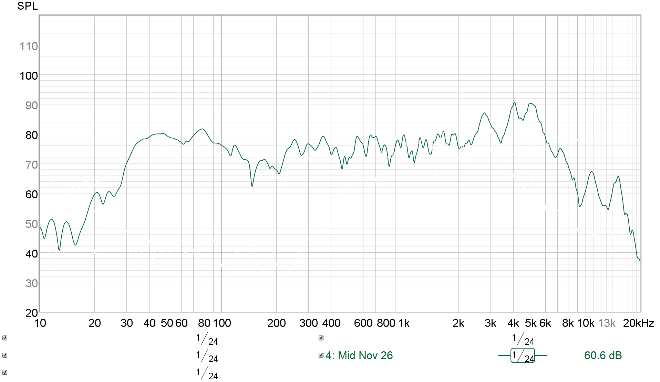
\includegraphics[width = 3 in]{Images/sp_spl_resp_mid.png}}
\qquad
\subfloat[\centering Tweeter Response]{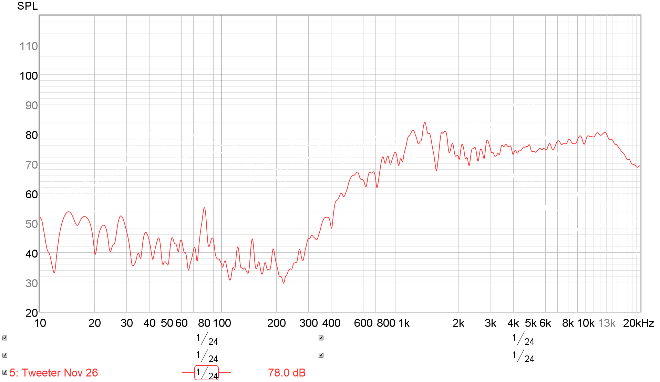
\includegraphics[width = 3 in]{Images/sp_spl_resp_tweeter.png}}
\qquad
\subfloat[\centering Subwoofer Response]{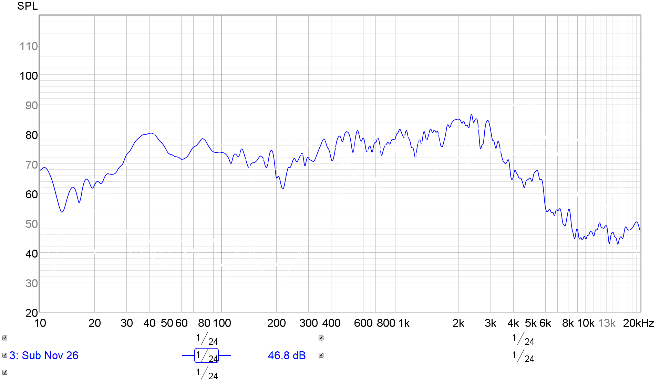
\includegraphics[width = 3 in]{Images/sp_spl_resp_sub.png}}
\caption{SPL Resonse of individual drivers after being installed int cabinet. Absolute values are uncallibrated, but relative intensities should be considered.}
\label{fig:sp_measured_SPL_resp}
\end{figure}
%
For completeness, the impedance of each driver was measured under fully installed conditions. Testing methodology was the same as described previously for SPL levels. The second impedance peak of the subwoofer at \SIrange{30}{40}{\hertz}. Is not predicted by the datasheet and may be attributed to the cabinet or the added mass. Similarly, the impedance peak at \SI{30}{\hertz} seen in the mid-bass is not predicted. The subsequent peaks may be predicted, the graph provided on the datasheet is of limited quality. The datasheet for the tweeter suggests a peak in the \SIrange{1.0}{1.5}{\kilo\hertz} range is to be expected. The impact of the series capacitance is clearly visible below \SI{300}{\hertz}. Data for below \SI{1}{\kilo\hertz} is not reported. Responses are presented as \Figure{sp_impedance}.\par
%
\begin{figure}[h!]
\centering
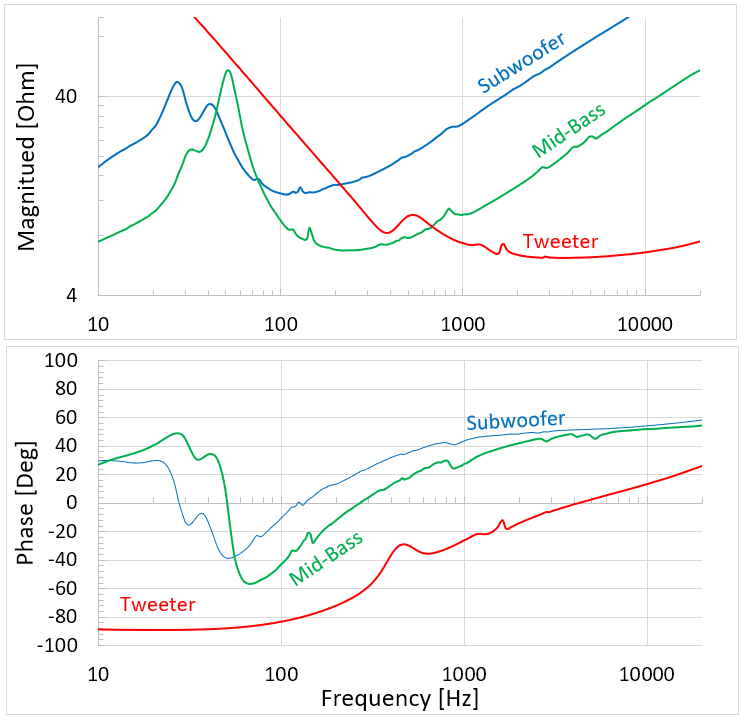
\includegraphics[height = 3.5 in]{Images/sp_dats_impedance_response.png}
\caption{Impedance measurements of individual drivers installed into the loudspeaker.}
\label{fig:sp_impedance}
\end{figure}
%
Neglecting gain, the preliminary filter configuration was as exculsively implemented as Butterworth filters. The low pass is a 2nd order (\SI{12}{\dB\per\oct}) filter with a \SI{200}{\hertz} cut-off, \SI{4}{\dB} of gain is applied to the output. The band pass consists of a 2nd order high-pass with a \SI{100}{\hertz} cut-off and a 4th order (\SI{24}{\dB\per\oct}) lowpass with a \SI{2}{\kilo\hertz} cut-off. The output of the bandpass is inverted in phase. The high-pass filter employs a 4th order filter with \SI{1}{\kilo\hertz} cut off. Half a \si{\dB} of gain is applied to the output of the high pass. With this minimal tuning a reasonably flat frequency response was measured, see \Figure{sp_early_dsp}.\par
%
\begin{figure}[h!]
\centering
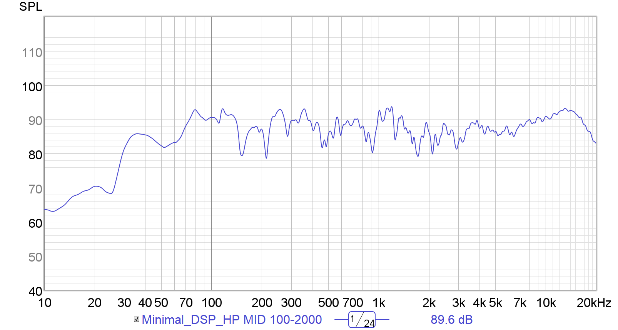
\includegraphics[height = 3.5 in]{Images/sp_spl_combined_prelim.png}
\caption{Measured frequency response of loudspeaker system using commercial digital signal processing modules for active crossover. Results are preliminary.}
\label{fig:sp_early_dsp}
\end{figure}
%
\section{Amplifier Design}
%

\end{document}
